\documentclass{beamer}
\beamertemplatenavigationsymbolsempty
\usecolortheme{beaver}
\setbeamertemplate{blocks}[rounded=true, shadow=true]
\setbeamertemplate{footline}[page number]
%
\usepackage[utf8]{inputenc}
\usepackage[english,russian]{babel}
\usepackage{amssymb,amsfonts,amsmath,mathtext}
\usepackage{subfig}
\usepackage[all]{xy} % xy package for diagrams
\usepackage{array}
\usepackage{multicol} % many columns in slide
\usepackage{hyperref} % urls
\usepackage{hhline} %tables
\usepackage{comment} %comments
\usepackage{adjustbox}
\newcommand{\blambda}{\boldsymbol{\lambda}}

\DeclareMathOperator*{\argmin}{arg\,min}
\DeclareMathOperator*{\argmax}{arg\,max}

% Your figures are here:
\graphicspath{ {../figures/} }

%----------------------------------------------------------------------------------------------------------

\title[\hbox to 56mm{Дистилляция знаний в глубоких сетях с применением методов выравнивания структур моделей}]{Дистилляция знаний в глубоких сетях с применением методов выравнивания структур моделей}
\subtitle{\textcolor{black}{Выпускная квалификационная работа бакалавра}}
\author[М.\,С.~Олейник]{
    Михаил Сергеевич Олейник\\
    Научный руководитель: к.ф.-м.н. О.\,Ю.~Бахтеев
}
\institute[МФТИ (НИУ)]{
\small{
    Кафедра интеллектуальных систем ФПМИ МФТИ\\
    Специализация: Интеллектуальный анализ данных\\
    Направление: 01.03.02 Прикладная математика и информатика
}}
\date{2024}


%----------------------------------------------------------------------------------------------------------
\begin{document}
%----------------------------------------------------------------------------------------------------------

\begin{frame}

    \thispagestyle{empty}
    \maketitle

\end{frame}

%-----------------------------------------------------------------------------------------------------

\begin{frame}{Актуальность исследования}

    \textbf{Проблема}: если модели ученика и учителя имеют сильно отличающиеся архитектуры, то сложно провести дистилляцию знаний.
    Есть методы, с помощью которых это возможно сделать, но они дают малый прирост качества.

    \bigskip

    \textbf{Цель}: предложить метод дистилляции, который будет работать для разных архитектур, с разным количеством слоёв,
    и показывать лучшее качество.

\end{frame}

%----------------------------------------------------------------------------------------------------------

\begin{frame}{Идея метода}

    \begin{columns}[c]
        \column{0.4\textwidth}
        \begin{figure}
            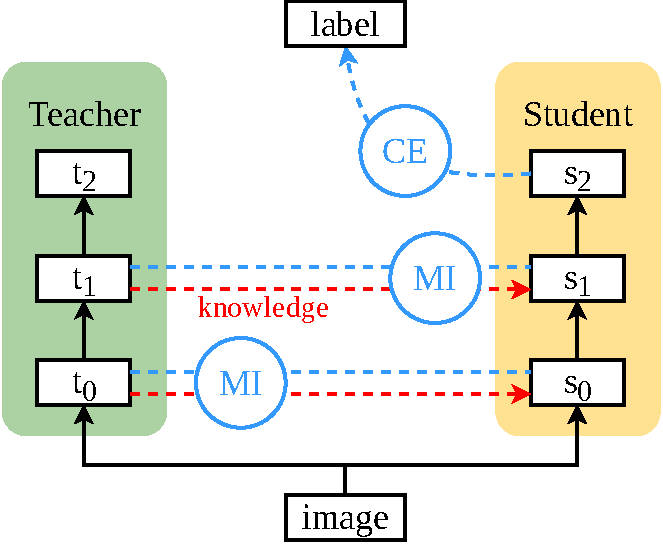
\includegraphics[width=1.0\textwidth]{ahn_diagram.pdf}
            \caption*{Метод Sungsoo Ahn \footnotemark}
        \end{figure}

        \column{0.4\textwidth}
        \begin{figure}
            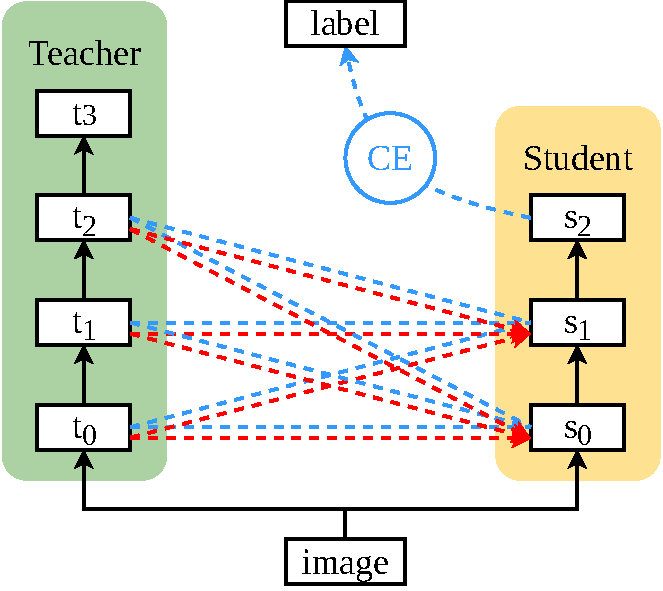
\includegraphics[width=1.0\textwidth]{our_diagram.pdf}
            \caption*{Наш метод}
        \end{figure}
    \end{columns}

    Слои объединяются не попарно, а каждый с каждым.

    \footnotetext[1]{Sungsoo Ahn et al. "Variational information distillation for knowledge transfer"}
\end{frame}

%----------------------------------------------------------------------------------------------------------

\begin{frame}{Постановка задачи классификации}
    Дана выборка для задачи классификации на $K$ классов:

    $$\mathfrak{D}  = \{(\bold{x}_i, y_i)\}_{i=1}^{m},\; \bold{x}_i \in \mathbb{R}^n,\; y_i \in \mathbb{Y}  = \{1, \dots, K\},$$
    где $\bold{x}_i$ --- данные, описывающие объект, взятые из распределения $p(\bold{x})$.

    Обозначим:
    \begin{itemize}
        \item $T$ --- количество слоев в модели учителе,
        \item $S$ --- количество слоев в модели ученике,
        \item $\bold{t}_{i}$ --- активации в $i$-м слое учителя,
        \item $\bold{s}_{i}$ --- активации в $i$-м слое ученика.
    \end{itemize}
\end{frame}


%----------------------------------------------------------------------------------------------------------

\begin{frame}{Функция потерь ученика с дистилляцией}
    Функцию потерь ученика представим как:
    $$
        \mathcal{L} = \beta \mathcal{L}_\text{CE} - (1 - \beta){\sum_{i=1}^T \sum_{j=1}^S \lambda_{i, j}\textcolor{red}{I(\bold{t}_{i}, \bold{s}_{j})}},
    $$
    где:
    \begin{itemize}
        \item $\mathcal{L}_\text{CE}$ --- функция потерь для решения задачи классификации (кросс-энтропия),
        \item $\textcolor{red}{I(\bold{t}_{i}, \bold{s}_{j})}$ --- взаимная информация,
        \item $\beta \in (0;1)$ и $\lambda_{i, j} \in [0;1]$ --- необучаемые параметры (гиперпараметры).
    \end{itemize}
\end{frame}



%----------------------------------------------------------------------------------------------------------

\begin{frame}{Максимизация взаимной информации}
    Метод вариации нижней границы:
    \begin{multline}
        I(\bold{t}; \bold{s}) = H(\bold{t}) - H(\bold{t} | \bold{s}) =  H(\bold{t}) + \mathbb{E}_{\bold{t},\bold{s}}[\log{p(\bold{t}|\bold{s})}] \\
        = H(\bold{t}) + \mathbb{E}_{\bold{t},\bold{s}}[\log{q(\bold{t}|\bold{s})}] + \mathbb{E}_{\bold{s}}[D_{\text{KL}}(p(\bold{t}|\bold{s})||q(\bold{t}|\bold{s}))] \\
        \geq H(\bold{t}) + \mathbb{E}_{\bold{t},\bold{s}}[\textcolor{red}{\log{q(\bold{t}|\bold{s})}}].
    \end{multline}
    Вид вариационного распределения, если слой $t$ --- свёрточный:
    \begin{multline}
        -\textcolor{red}{\log{q(t|s)}} = -\sum_{c=1}^{C}  \sum_{h=1}^{H} \sum_{w=1}^{W} \log{q(t_{c,h,w}|s)} = \\
        = \sum_{c=1}^{C}  \sum_{h=1}^{H} \sum_{w=1}^{W} \log{\textcolor{blue}{\sigma_c}} + \frac{(t_{c,h,w} - \textcolor{blue}{\mu_{c,h,w}(s)})^2}{2\textcolor{blue}{\sigma_c}^2} + constant.
    \end{multline}
\end{frame}

%-----------------------------------------------------------------------------------------------------

\begin{frame}{Постановка двухуровневой оптимизации}
    $$\mathfrak{D} = \mathfrak{D}_\text{train} \bigsqcup \mathfrak{D}_\text{val}.$$
    Определим вектор $\blambda$ из всех гиперпараметров задачи:
    $$\blambda = [\lambda_{0, 0}, \ldots, \lambda_{i, j}, \ldots, \beta].$$

    Все обучаемые параметры --- $\bold{w}$.

    И это определяет задачу двухуровневой оптимизации:
    $$\min_{\blambda} \quad \mathcal{L}_\text{val}(\bold{\hat{w}}(\blambda), \blambda),$$
    $$\text{s.t.} \quad  \bold{\hat{w}}(\blambda) = \argmin_{\bold{w}}{\mathcal{L}_\text{train}(\bold{w}, \blambda)}. $$

\end{frame}

%-----------------------------------------------------------------------------------------------------

\begin{frame}{Данные вычислительного эксперимента}
    \begin{table}[h!]
        \centering
        \begin{adjustbox}{max width=\textwidth}
            \begin{tabular}{|c|c|}
                \hline
                Tiny                                                  & VeryTiny                                              \\
                \hline \hline
                Свёрточный 2D слой \break ($3 \times 3$, 4 фильтра)   & Свёрточный 2D слой \break ($3 \times 3$, 8 фильтров)  \\ \hline
                Свёрточный 2D слой \break ($3 \times 3$, 8 фильтров)  & Свёрточный 2D слой \break ($3 \times 3$, 16 фильтров) \\ \hline
                Свёрточный 2D слой \break ($3 \times 3$, 16 фильтров) & Свёрточный 2D слой \break ($3 \times 3$, 32 фильтра)  \\ \hline
                Полносвязный слой  \break (64 нейрона)                & Полносвязный слой \break (64 нейрона)                 \\ \hline
                Полносвязный слой  \break (10 нейронов)               & Полносвязный слой \break (10 нейронов)                \\ \hline
            \end{tabular}
        \end{adjustbox}
        \caption*{Архитектура моделей Tiny и VeryTiny, слои заданы поочередно, сверху вниз}
        \label{table:model_scheme}
    \end{table}
    \begin{columns}[c]
        \column{0.5\textwidth}
        Датасеты:
        \begin{itemize}
            \item CIFAR10
            \item FashionMNIST
        \end{itemize}
        \column{0.5\textwidth}
        Модели:
        \begin{itemize}
            \item Учитель: Tiny
            \item Ученик: VeryTiny
        \end{itemize}
    \end{columns}

\end{frame}

%----------------------------------------------------------------------------------------------------------

\begin{frame}{Результаты эксперимента}
    Метрика качества: точность. \\

    \begin{table}[h!]
        \centering
        \begin{adjustbox}{max width=\textwidth}
            \begin{tabular}{|c|c|c|}
                \hline
                Метод                                & CIFAR-10       & Fashion-MNIST  \\
                \hline \hline
                Без дистилляции                      & $0.541$        & $0.839$        \\ \hline
                Дистилляция Хинтона                  & $0.563$        & $0.849$        \\ \hline
                Дистилляцией Sungsoo Ahn             & $0.591$        & $0.852$        \\ \hline
                Наш метод, все связи                 & $0.590$        & $0.853$        \\ \hline
                Наш метод, случайные гиперпараметры  & $0.595$        & $\bold{0.859}$ \\ \hline
                Наш метод, вероятностная оптимизация & $\bold{0.608}$ & $0.857$        \\ \hline
            \end{tabular}
        \end{adjustbox}
        \caption*{Значение качества экспериментов на датасетах CIFAR-10 и Fashion-MNIST}
        \label{table:result_accuracy}
    \end{table}
\end{frame}

%----------------------------------------------------------------------------------------------------------

\begin{frame}{Дальнейшие исследования}
    \begin{figure}[H]
        \begin{minipage}[h]{0.35\linewidth}
            \center{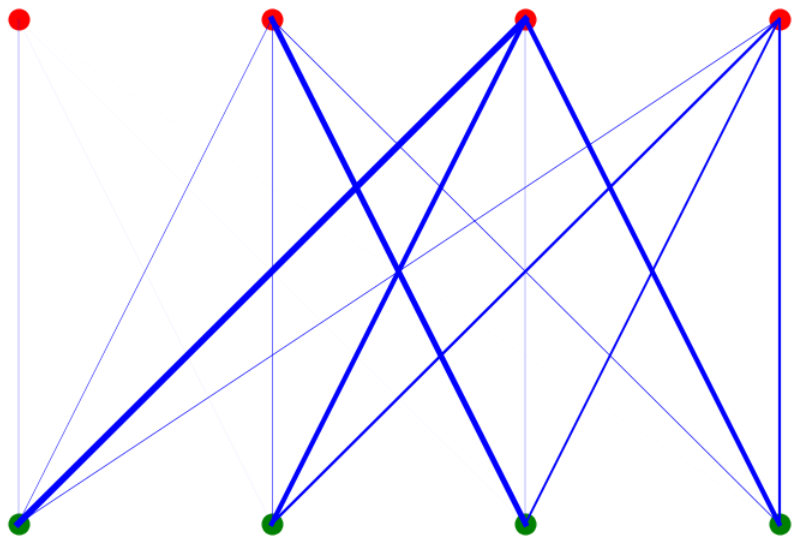
\includegraphics[width=1\linewidth]{connections_1}} a) \\
        \end{minipage}
        \hfill
        \begin{minipage}[h]{0.35\linewidth}
            \center{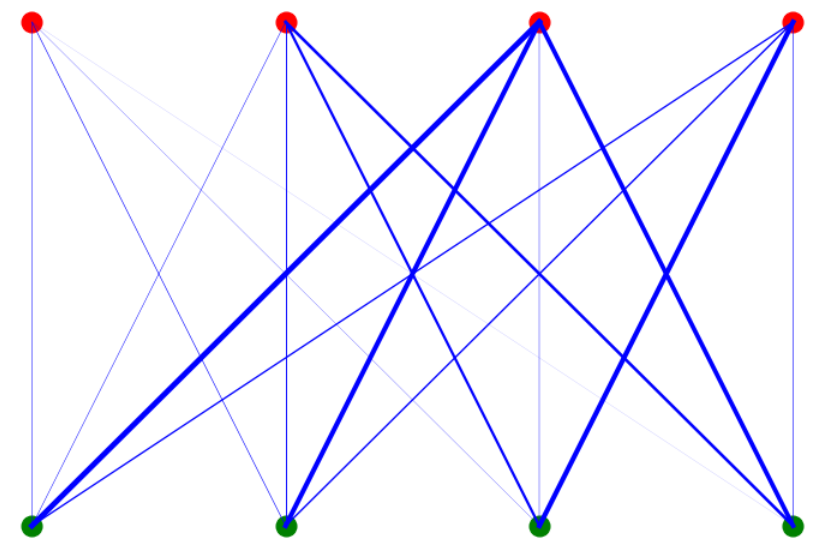
\includegraphics[width=1\linewidth]{connections_2}} b) \\
        \end{minipage}
        \vfill
        \begin{minipage}[h]{0.35\linewidth}
            \center{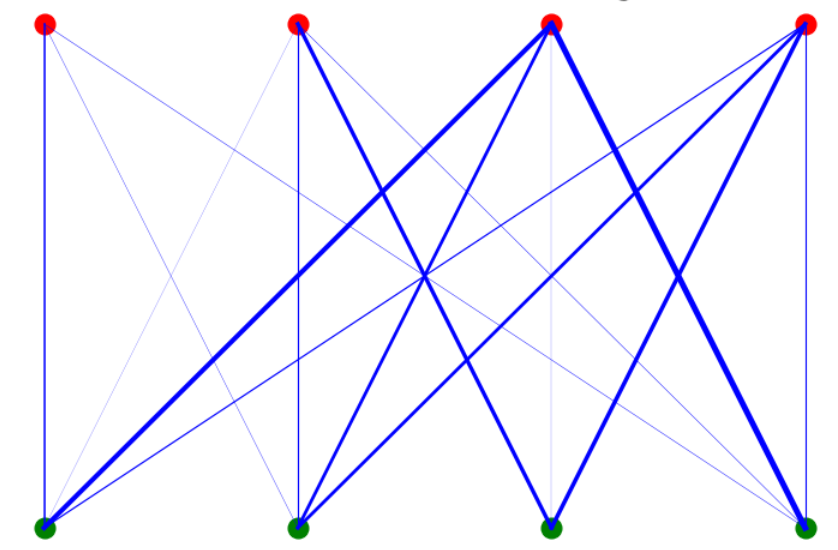
\includegraphics[width=1\linewidth]{connections_3}} c) \\
        \end{minipage}
        \hfill
        \begin{minipage}[h]{0.35\linewidth}
            \center{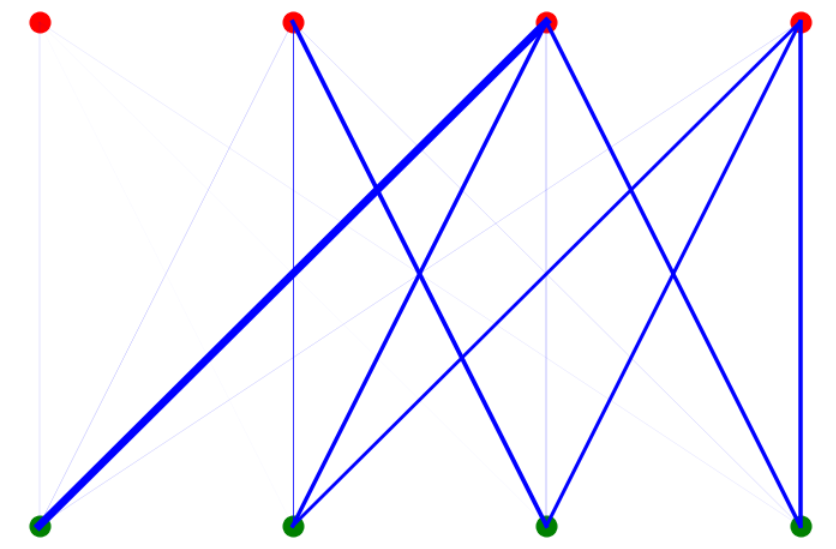
\includegraphics[width=1\linewidth]{connections_4}} d) \\
        \end{minipage}
        \caption{Иллюстрация коэффициентов у четырех лучших моделей по качеству. Зелёные точки --- слои ученика, красные --- слои учителя. Чем толще линия, тем больше коэффициент у соответствующей связи.}
    \end{figure}
\end{frame}

%----------------------------------------------------------------------------------------------------------

\begin{frame}{Выносится на защиту}
    \begin{itemize}
        \item Предложен метод дистилляции, максимизирующий взаимную информацию между всеми слоями ученика и учителя.
        \item Продемонстрировано, что предложенный метод достигает лучшего качества, чем базовые методы дистилляции знаний.
        \item Были проведены эксперименты, показавшие эффективность предложенного метода.
    \end{itemize}
\end{frame}

%----------------------------------------------------------------------------------------------------------
\end{document}